\documentclass[../../main.tex]{subfiles}

\begin{document}

\subsection{Class diagram}

A UML class diagram describing the main entities involved in the system follows.
Customers use the system to line up in the queue of a store and obtain a line up
receipt, which will grant them a visit to the store. Each store belongs to a given
chain of stores. Moreover, each store can be internally divided in departments,
containing different categories of purchasable items. When the customers line
up, they can specify the categories of items they intend to buy. Finally, the
system knows the locations of the customers and of the stores.

The line up receipt is represented by a QR code for the customers that interact with the system with an IT device.

If the customers interact with the system using a standard telephone line, they are given a numeric code as a representation of the line up receipt, which they will be able to convert to a printed QR code line up receipt thanks to the store assistants outside of the store.

The customers who interact with the system in presence request the printed QR code line up receipt directly to the store assistants outside of the store.

\begin{figure}[H]
    \centering
    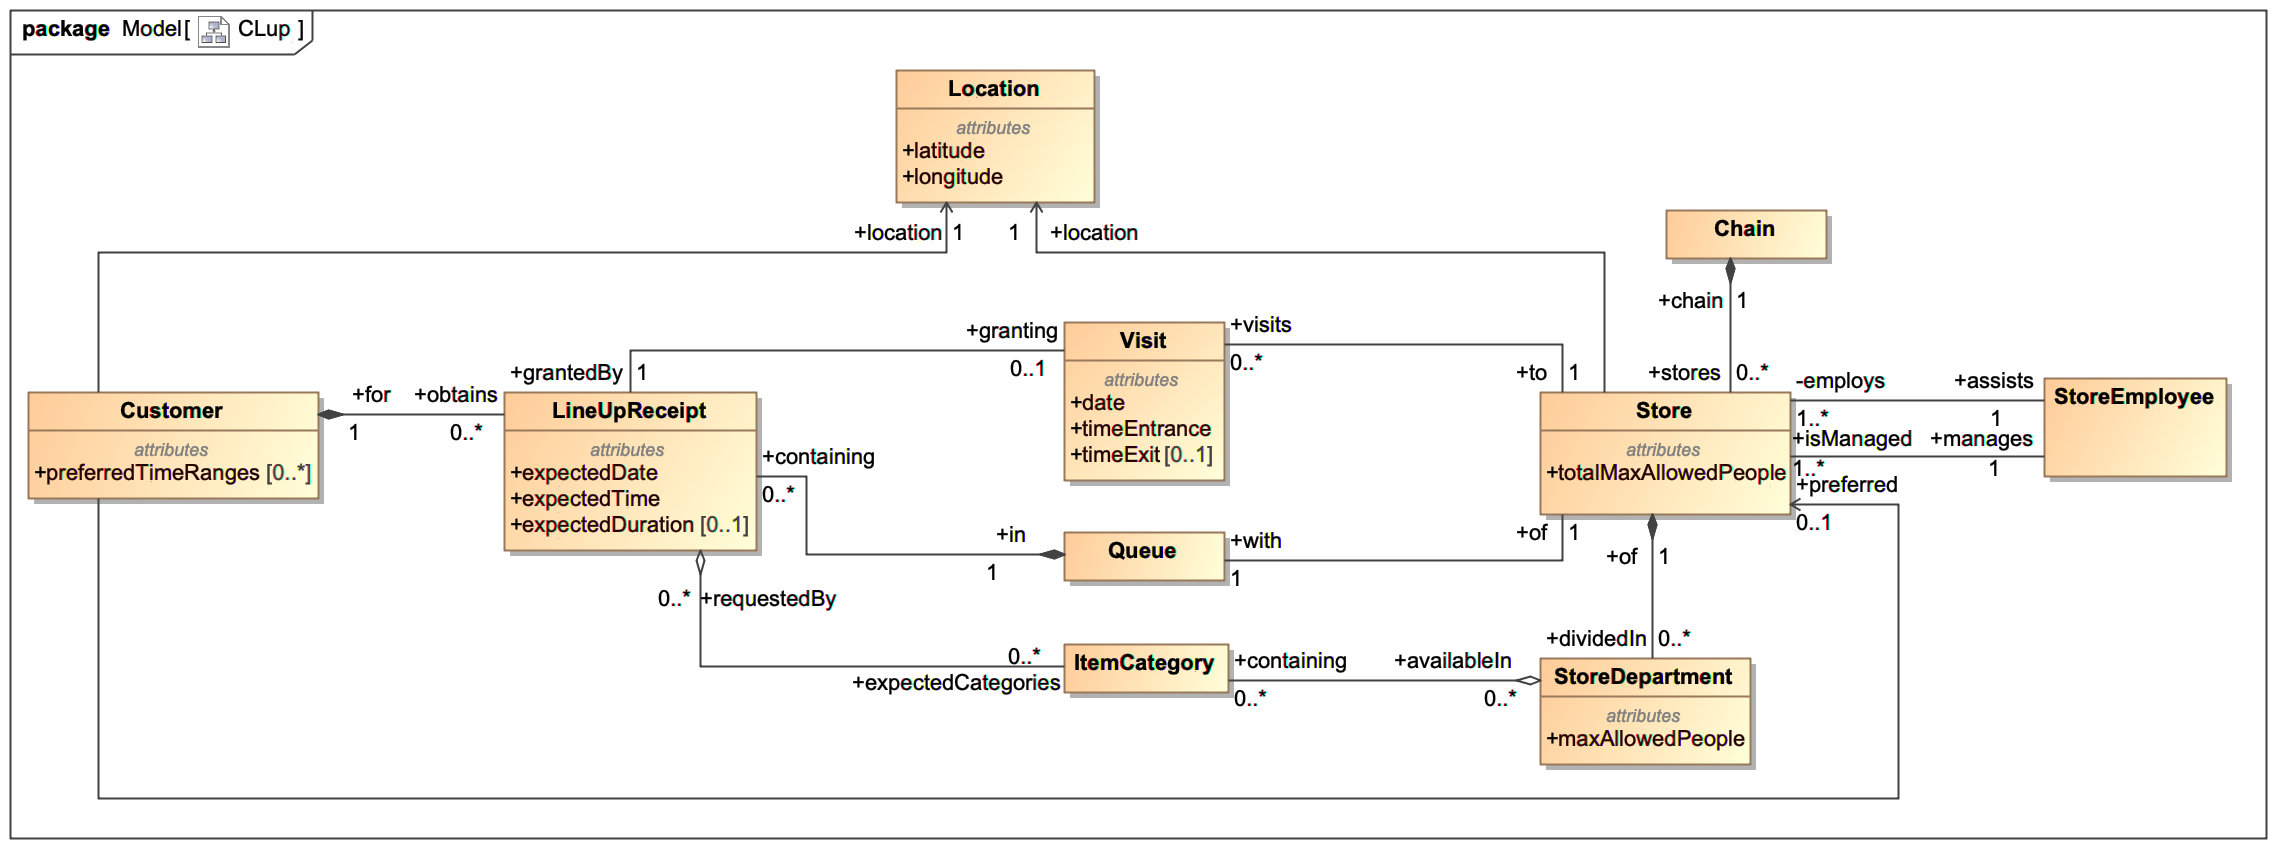
\includegraphics[width=\textwidth]{class__CLup.png}
    \caption{The class diagram of CLup's application domain.}
\end{figure}

\subsection{State chart diagrams}

The internal state of the main entities of the domain is better defined in the following UML
state diagrams.

\begin{figure}[H]
    \centering
    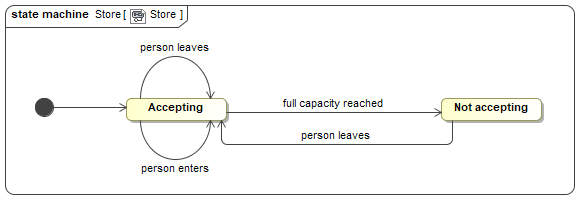
\includegraphics[width=\textwidth]{stm__Store__Store.png}
    \caption{Statechart of a store in the application domain.}
\end{figure}

\begin{figure}[H]
    \centering
    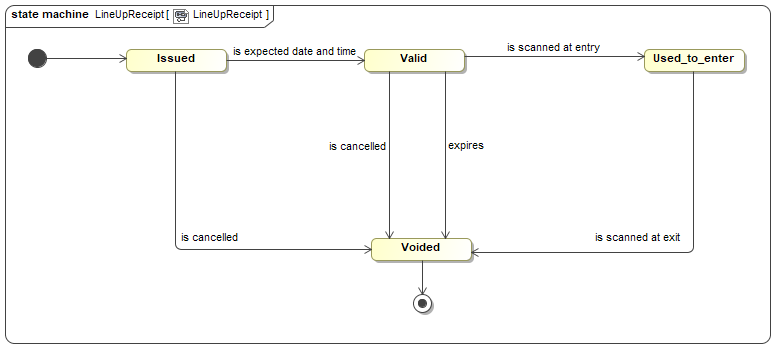
\includegraphics[width=\textwidth]{stm__LineUpReceipt__LineUpReceipt.png}
    \caption{Statechart of a lineup receipt in the application domain.}
\end{figure}

\subsection{Scenarios}

\newcounter{ScenarioCounter}

\stepcounter{ScenarioCounter}
\subsubsection{Scenario \arabic{ScenarioCounter}}

  Luca lives in a country where lockdown policies are applied. The last time he shopped for groceries online, 
  he forgot to add to the cart olive oil, and now he needs it. Waiting until the next delivery would take too much time, 
  so Luca decides to line up for the nearest store. 
  Luca opens CLup, looks for the nearest store and selects it. 
  He then inserts the expected duration of his visit and the category of the item he wants to buy. 
  Unfortunately, CLup estimates that the olive oil department will be busy for the next hours. 
  CLup suggests an alternative store in proximity, where there is a free slot sooner. 
  Luca accepts the suggestion and CLup queues Luca to access the store. Luca receives confirmation.

\stepcounter{ScenarioCounter}
\subsubsection{Scenario \arabic{ScenarioCounter}}

  Anna, a long time customer of the local store, wants to reserve a time slot to go grocery shopping the next week. 
  Anna opens CLup and selects the desired store and the desired date and time slot. 
  Not knowing yet which articles she might need, she does not fill the product categories section, 
  and she does not provide any visit duration estimation. Once Anna confirms her intentions to CLup, 
  the system predicts automatically the duration and the departments she is most likely to be in, 
  based on the collected history of previous visits. CLup then checks if Anna's visit is compatible with the 
  current schedule of the store, and, as the answer is positive, it shows a confirmation of the reservation to Anna.

\stepcounter{ScenarioCounter}
\subsubsection{Scenario \arabic{ScenarioCounter}}

  Maurizio reserved a slot in the queue to access the nearby store through CLup, but, due to an unforeseen commitment, 
  he has to cancel the appointment. Maurizio opens CLup, selects the reservation and cancels it. 
  The system removes Maurizio from the queue and sends a confirmation to the customer. 
  Meanwhile, Patrizia wanted to access the store as soon as possible, but all the nearest time slots were busy, 
  and the system delayed her reservation. CLup, aware of the recently freed time slot, sends a notification to Patrizia offering her to take it over. 
  Patrizia opens CLup, accepts the offering and CLup queues her in the time slot.


\stepcounter{ScenarioCounter}
\subsubsection{Scenario \arabic{ScenarioCounter}}

  Alina is in line through CLup to access a store and her visit start time is near. 
  CLup sends a notification to Alina to remind her of the visit. 
  Alina departs from her home and approaches the store, showing the receipt on her IT device to the receipt scanner. 
  CLup checks if the customer arrived either too early or too late with respect to the assigned time slot. 
  Alina is perfectly in time and is allowed to enter the store. Finally, when the visit is coming to an end, 
  Alina's receipt is shown once again at the store cashier, who scans it. 
  CLup registers the end of the visit and sends a confirmation message to the cashier.


\stepcounter{ScenarioCounter}
\subsubsection{Scenario \arabic{ScenarioCounter}}

  Alessandro, a nurse, would like to stop at the store on the way home from work to do some urgent grocery shopping. 
  Unfortunately, Alessandro's smartphone is out of charge, and he cannot use CLup. 
  Alessandro stops at the store anyway, approaches the store assistant at the entrance, and asks for a receipt. 
  The store assistant accesses CLup and requests to queue a visitor. The system adds the customer to the queue and sends the line up receipt as a confirmation. 
  The store assistant prints the line up receipt and gives it to Alessandro, who waits his turn.



\stepcounter{ScenarioCounter}
\subsubsection{Scenario \arabic{ScenarioCounter}}

  Andrea does not own either a smartphone or a personal computer. 
  Andrea would want to queue up immediately to go grocery shopping in a store adopting the CLup system, 
  but, as he is missing any IT device, he can not access the system through the Internet. 
  Andrea calls CLup's number, and the system guides him through the process: first of all, 
  the synthesized voice asks Andrea if he would like to access the store as soon as possible or to reserve a time slot, 
  and then the store he would like to visit. Once Andrea has answered the questions and confirmed his intentions, 
  the system adds Andrea to the queue of the store. The system then dictates the numeric code to be used at the entrance of the store. 
  Once Andrea confirms that he has understood the code, the interaction is closed.



\stepcounter{ScenarioCounter}
\subsubsection{Scenario \arabic{ScenarioCounter}}

  This time, Andrea would want to reserve a time slot to go grocery shopping next week. 
  Andrea calls CLup's number and states, once asked, that he would like to use the reservation functionalities. 
  CLup asks Andrea, in sequence, which store he would like to access, at what date, and at which time. 
  The system repeats Andrea's choices and asks for confirmation. Once Andrea confirms, 
  the system estimates the visit duration and checks if it is compatible with the current schedule. 
  The system then dictates the numeric code to be used at the entrance of the store. 
  Once Andrea confirms that he has understood the code, the interaction is closed.

  The following week Andrea gets a call from CLup, as a notification for the incoming visit. 
  As Andrea approaches the store, he goes to the store assistant, and shows her the numeric code 
  for the visit.
  The store assistant accesses CLup, and provides the system the numeric code. 
  The system gives a successful response to the store assistant, who then prints the ticket valid 
  for the visit and hands it to Andrea. 
  Now Andrea can access the store and do the shopping.



\stepcounter{ScenarioCounter}
\subsubsection{Scenario \arabic{ScenarioCounter}}

  Michael is a store manager at a famous supermarket chain, in a country in which COVID 
  restrictions are in effects.
  One day, the country's government releases new safety standards for supermarkets safety, which 
  includes the maximum amount of people per squared meter who can access the store. 
  The next day, before the store opening, Michael needs to update its safety parameters with the 
  newly defined ones. 
  To do this, Michael accesses CLup system, and then requests to update the safety parameters. 
  The system asks Michael for the confirmation and he confirms. 
  The system now saves the new parameters, and puts them into effect, modifying the store queue 
  availability.



\stepcounter{ScenarioCounter}
\subsubsection{Scenario \arabic{ScenarioCounter}}

  The same day Michael set the new safety parameters, the authorities come into his supermarket, 
  asking for the supermarket's statistics about customers flux inside the supermarket. 
  Michael accesses CLup system, and then requests to see the required statistics. 
  The system provides the requested statistics, and Michael hands them to the authorities. 

\end{document}
